\documentclass[border=5pt]{standalone}
\usepackage{tikz}
\usetikzlibrary{shapes}


\tikzset{
  image/.pic={
    \node[circle,draw,inner sep=0pt,minimum size=2pt] (a) at (0,0) {};
    \node[circle,draw,inner sep=0pt,minimum size=2pt] (b) at (1/2, -1.658) {};
    \node[circle,draw,inner sep=0pt,minimum size=2pt] (c) at (-1/2, -1.658) {};

    \node[circle,draw,inner sep=0pt,minimum size=2pt] (d) at (0.7287, -0.685) {};
    \node[circle,draw,inner sep=0pt,minimum size=2pt] (e) at (-0.2287, -0.9735) {};
    \node[circle,draw,inner sep=0pt,minimum size=2pt] (f) at (0.2287, -0.9735) {};

    \node[circle,draw,inner sep=0pt,minimum size=2pt] (g) at (-0.7287, -0.685) {};


    \draw[thick] (a) -- (d); 
    \draw[thick] (a) -- (e); 
    \draw[thick] (a) -- (f);
    \draw[thick] (a) -- (g);  
    
    \draw[thick] (b) -- (c); 
    \draw[thick] (b) -- (d); 
    \draw[thick] (b) -- (e);
    
    \draw[thick] (c) -- (f);
    \draw[thick] (c) -- (g);
    
    \draw[thick] (d) -- (e);
    \draw[thick] (f) -- (g);
  }
}

\begin{document}
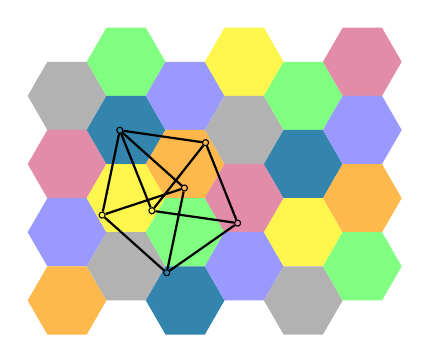
\begin{tikzpicture} [hexa/.style= {shape=regular polygon,
                                   regular polygon sides=6,
                                   minimum size=1cm, draw=none,
                                   inner sep=0,anchor=south,
                                   fill=lightgray!85!blue}]



\node[hexa, fill=black!30!white] at ({3/2+3/4},{(4+1/2)*sin(60)}) {};
\node[hexa, fill=purple!45!white] at ({3/2+3/4},{(3+1/2)*sin(60)}) {};
\node[hexa, fill=blue!40!white] at ({3/2+3/4},{(2+1/2)*sin(60)}) {};
\node[hexa, fill=red!40!yellow!70!white] at ({3/2+3/4},{(1+1/2)*sin(60)}) {};

\node[hexa, fill=green!50!white] at ({4/2+4/4},{(5)*sin(60)}) {};
\node[hexa, fill=green!40!blue!80!white] at ({4/2+4/4},{(4)*sin(60)}) {};
\node[hexa, fill=yellow!70!white] at ({4/2+4/4},{(3)*sin(60)}) {};
\node[hexa, fill=black!30!white] at ({4/2+4/4},{(2)*sin(60)}) {};

\node[hexa, fill=blue!40!white] at ({5/2+5/4},{(4+1/2)*sin(60)}) {};
\node[hexa, fill=red!40!yellow!70!white] at ({5/2+5/4},{(3+1/2)*sin(60)}) {};
\node[hexa, fill=green!50!white] at ({5/2+5/4},{(2+1/2)*sin(60)}) {};
\node[hexa, fill=green!40!blue!80!white] at ({5/2+5/4},{(1+1/2)*sin(60)}) {};

\node[hexa, fill=yellow!70!white] at  ({6/2+6/4},{(5)*sin(60)}) {};
\node[hexa, fill=black!30!white] at ({6/2+6/4},{(4)*sin(60)}) {};
\node[hexa, fill=purple!45!white] at ({6/2+6/4},{(3)*sin(60)}) {};
\node[hexa, fill=blue!40!white] at ({6/2+6/4},{(2)*sin(60)}) {};

\node[hexa, fill=green!50!white] at ({7/2+7/4},{(4+1/2)*sin(60)}) {};
\node[hexa, fill=green!40!blue!80!white] at ({7/2+7/4},{(3+1/2)*sin(60)}) {};
\node[hexa, fill=yellow!70!white] at ({7/2+7/4},{(2+1/2)*sin(60)}) {};
\node[hexa, fill=black!30!white] at ({7/2+7/4},{(1+1/2)*sin(60)}) {};

\node[hexa, fill=purple!45!white] at  ({8/2+8/4},{(5)*sin(60)}) {};
\node[hexa, fill=blue!40!white] at ({8/2+8/4},{(4)*sin(60)}) {};
\node[hexa, fill=red!40!yellow!70!white] at ({8/2+8/4},{(3)*sin(60)}) {};
\node[hexa, fill=green!50!white] at ({8/2+8/4},{(2)*sin(60)}) {};


\pic[rotate=35,transform shape,scale=1.1] at (2.92,3.9) {image};

\end{tikzpicture}
\end{document}
